% !TEX encoding = UTF-8 Unicode
% ------------------------------------------------------------------------------
% Este fichero es parte de la plantilla LaTeX para la realización de Proyectos
% Final de Grado, protegido bajo los términos de la licencia GFDL.
% Para más información, la licencia completa viene incluida en el
% fichero fdl-1.3.tex

% Copyright (C) 2012 SPI-FM. Universidad de Cádiz
% ------------------------------------------------------------------------------

Las instrucciones de instalación y explotación del sistema se detallan a continuación.

\section{Introducción}

El presente software está destinado a la gestión de un centro de mejora de la salud y el rendimiento, en concreto, ha sido una personalización para el centro \textit{CoreSport}, en Chiclana de la Frontera (Cádiz). \\

Cualquier centro similar que precise de un software de gestión puede hacer uso del mismo con o sin modificaciones, bajo la licencia GNU GPL (Licencia Pública General de GNU) en su versión 3 o superior (\ref{GNU-license}). 


\section{Requisitos previos}

Ha de diferenciarse dos tipos de usos o instalaciones del sistema: 

\begin{itemize} 
\item Sin modificaciones: Si se pretende hacer uso del software tal y como se entrega, sin necesidad de un desarrollo previo para su modificación o ampliación, habría que hacer uso de un servidor para la instalación de \textit{GlassFish} o \textit{WildFly (JBoss)} (recomendado), o cualquier otro servidor de aplicaciones compatible para, posteriormente, realizar la instalación del software. Para ello, bastaría con el archivo \textit{Booking.ear} contenido en el directorio \textit{dir}, el cual se puede cargar directamente en el servidor, junto con el backup de la base de datos con los datos básicos para poder iniciar el sistema. Se añadirá un manual de instalación para entornos de producción en un futuro cercano. 
\item También sería posible, una vez el sistema se encuentre en producción, utilizar el mismo servidor para varias empresas, lo que facilitaría la instalación -ya estaría hecha- y reduciría el precio del servicio al ser compartido. En este caso, solo habría que añadir la nueva organización y sus elementos para la interfaz (logo, icono, estilo...). 
\item Instalación para desarrollo: En caso que se requiera una instalación local para desarrollo, la instalación sería diferente. Para ello, cualquier equipo básico con un rendimiento aceptable sería suficiente para la instalación. Respecto al software, haría falta, aparte del código del propio proyecto, la instalación de \textit{JDK, NetBeans, PostgreSQL, pgAdmin} y un servidor de aplicaciones, como \textit{GlassFish} (recomendado por su \textit{hot deployment}) o \textit{WildFly (JBoss)}, junto a los archivos \textit{jar} de \textit{Primefaces, PostgreSQL, Commons IO} y \textit{JavaEE Endorsed API}, librerías de las que se beneficiará el PFC.
\end{itemize} 


\section{Inventario de componentes}

Al descargar una copia del código fuente del PFC, se obtiene lo siguiente: 

\begin{itemize}
\item \textbf{Código fuente del proyecto}: Código Java de la aplicación web.
\item Últimas versiones disponibles -en septiembre de 2017- de los \textbf{archivos .jar} necesarios, contenidos en el directorio \textit{lib: Primefaces, PostgreSQL, Commons IO} y \textit{JavaEE Endorsed API}, además de los drivers de \textit{PostgreSQL} para \textit{GlassFish} (\textit{postgresql-9.3-1102.jdbc41.jar}).
\item Copia de una \textbf{base de datos} básica, con una organización, un superadministrador, un administrador y un cliente. Además de un \textbf{archivo explicativo} donde se facilitan los datos de estos usuarios y contraseñas y se explica cómo crear estos datos de forma personalizada. 
\item \textbf{Memoria del proyecto}, tanto en PDF como en \LaTeX, para que pueda ser actualizada si se desea. 
\end{itemize}


\section{Procedimientos de instalación}

A continuación se detallarán todos los pasos necesarios para la instalación del sistema en un equipo para su desarrollo o para pruebas locales. \\

Primeramente se procederá a la descarga de todos los elementos software necesarios: 

\begin{itemize}
\item \textit{JDK (Java Development Kit)} \cite{JDK}, que es el software que proporciona las herramientas para el desarrollo de aplicaciones Java.
\item \textit{NetBeans}, IDE (Entorno de Desarrollo Integrado) para el desarrollo de aplicaciones. Pensado principalmente para aplicaciones Java.
\item \textit{GlassFish}, servidor de aplicaciones para el desarrollo del proyecto en local.
\item \textit{Oracle} también ofrece la posibilidad de descargar \textit{NetBeans} con \textit{JDK8} -e incluso con \textit{GlassFish}- para que sea más cómodo y rápido \cite{NetBeans-con-JDK}.
\item Código fuente del proyecto, disponible en el repositorio \textit{GitHub} destinado a ello \cite{github-booking}.
\item \textit{PostgreSQL} \cite{PostgreSQL}, sistema de gestión de bases de datos a utilizar.
\item \textit{pgAdmin} \cite{pgAdmin}, interfaz de usuario para la administración de bases de datos PostgreSQL.
\item Librerías \textit{.jar} indicadas, que se encuentran en el directorio \textit{lib}, aunque se debe tener en cuenta la existencia de nuevas versiones. Las librerías serían:

\begin{itemize}
\item \textit{Commons IO}
\item \textit{Primefaces}
\item \textit{JavaEE Endorsed API}
\end{itemize}
\end{itemize}

\item El archivo .jar perteneciente al driver de \textit{PostgreSQL} para \textit{GlassFish: postgresql-9.3-1102.jdbc41.jar}.

Una vez descargado todo lo necesario, se procederá a la instalación de cada uno de ellos, junto a la creación y configuración del proyecto:

\begin{enumerate}
\item Se instalará \textit{NetBeans} con \textit{JDK} -actualmente JDK8-, ya sea en la misma instalación o por separados. 

\item Asimismo, se procederá a la instalación de \textit{GlassFish} si no se ha realizado en conjunto con la anterior. Si se hace por separado, habría que añadir el servidor a \textit{NetBeans} a través de la pestaña \textit{Services}, haciendo clic derecho en \textit{Servers} y añadiendo el servidor, eligiendo \textit{GlassFish} y a continuación la ruta donde se encuentra la carpeta descargada.  

\item Seguidamente, se creará un nuevo proyecto en \textit{NetBeans}:

\begin{enumerate}
\item Se elegirá la categoría \textit{Java EE} y el tipo de proyecto \textit{Enterprise Application with Existing Sources}, para crear el proyecto a partir del código fuente descargado. 

\begin{figure}[H]
\centering
  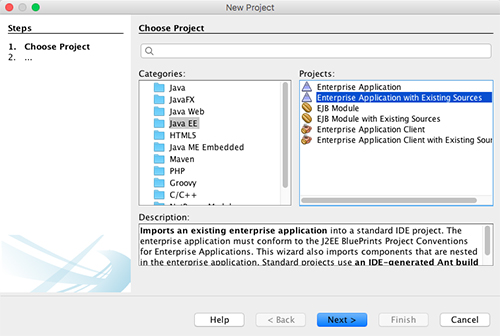
\includegraphics[scale=.60]{img/instalacion/nuevo-proyecto.jpg}
  \caption{\textit{Creación de un nuevo proyecto en NetBeans}}
  \label{fig:nuevo-proyecto}
\end{figure}

\item En el siguiente paso de la creación del proyecto, se selecciona la ubicación del mismo. Podemos cambiar el nombre y ubicación del proyecto en este paso, así como indicarle a \textit{NetBeans} cuál es el directorio que vamos a utilizar para almacenar las librerías que se van a usar activando la casilla \textit{Use Dedicated Folder for Storing Libraries}, como vemos en la figura \ref{fig:nuevo-proyecto}.

\begin{figure}[H]
\centering
  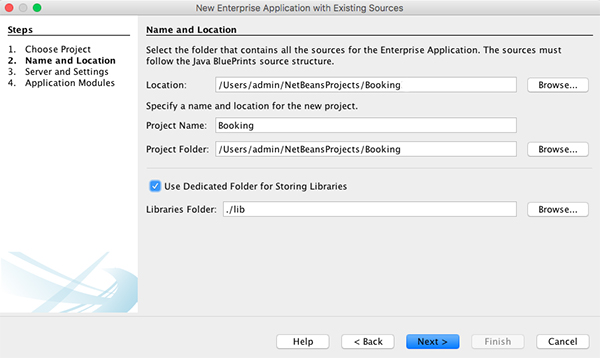
\includegraphics[scale=.55]{img/instalacion/ubicacion-nuevo-proyecto.jpg}
  \caption{\textit{Creación del proyecto: Ubicación}}
  \label{fig:ubicacion-nuevo-proyecto}
\end{figure}

\item En el próximo paso elegiremos el servidor de aplicaciones a emplear, en este caso \texti{GlassFish}, y la versión Java EE, eligiendo en ambas opciones su versión más reciente. 

\item Por último en cuanto a la creación del proyecto se refiere, se observa que el módulo Web \texti{Booking-war} se ha añadido automáticamente. Añadimos también el módulo EJB haciendo clic en la opción para ello y eligiendo el directorio \texti{Booking-ejb}. Una vez añadido, seleccionamos que se trata del módulo EJB, como vemos en la imagen \ref{fig:modulos-proyecto}.

\begin{figure}[H]
\centering
  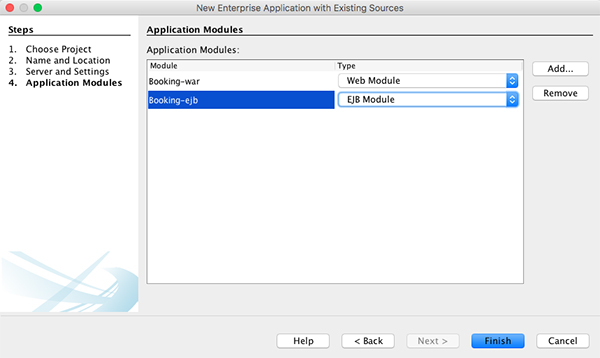
\includegraphics[scale=.55]{img/instalacion/modulos-proyecto.jpg}
  \caption{\textit{Definición de los módulos del proyecto}}
  \label{fig:modulos-proyecto}
\end{figure}

\end{enumerate}

\item Una vez el proyecto ha sido creado, definiremos dónde se encuentra nuestro módulo web a través del \textit{context root} del archivo \textit{application.xml} que encontraremos en el directorio \textit{Configuration Files} del proyecto. Cambiaremos la fila dedicada a ello, definiendo el \textit{context root} como sigue: \textit{<context-root/>}, de tal forma que le indicaremos al sistema que el módulo se encuentra en el directorio raíz, no haciendo falta ruta alguna para llegar a él.

\begin{figure}
\centering
  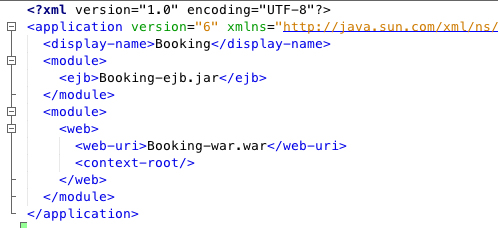
\includegraphics[scale=.65]{img/instalacion/context-root.jpg}
  \caption{\textit{Estableciendo el context root del archivo application.xml}}
  \label{fig:context-root}
\end{figure}

\item En este momento, se puede observar que existen diferentes advertencias de errores, las solucionaremos como sigue:

\begin{enumerate}
\item En el módulo \textit{Web} existen advertencias de errores, a través de iconos en los directorios donde estos aparecen; se trata de la falta de las librerías de las que el código hace uso. Por lo que seguidamente instalaremos estas dependencias del proyecto, es decir, las librerías \textit{Primefaces} y \textit{Commons IO}. Para ello, simplemente haremos clic secundario en el directorio \textit{Libraries} del módulo Web (\textit{Booking-war}) y seleccionamos la opción para añadir un archivo JAR (\textit{Add JAR/Folder...}). Seleccionamos una de las dos librerías y haremos seguidamente el mismo proceso para la otra. Observamos que los iconos de errores desaparecen. 

\item Asimismo, observamos que existe una advertencia similar, en este caso se informa que no se encuentra la librería \textit{JavaEE Endorsed API}, una de las dependencias del código. Para solucionarlo, abriremos la ventana de información, como vemos en la figura \ref{fig:advertencia-javaee-endorsed-api} y pulsaremos el botón \textit{Resolve...}. Aquí, añadiremos primeramente una nueva librería pulsando el botón \textit{New Library...} y asignándole el mismo nombre que nos pide: \textit{javaee-endorsed-api-7.0}, en este caso. Una vez creada, se añadirá el archivo \textit{jar} correspondiente a esta librería a través del botón \textit{Add JAR/Folder}. Una vez hecho esto, pulsaremos \textit{OK}.
\end{enumerate}

\begin{figure}
\centering
  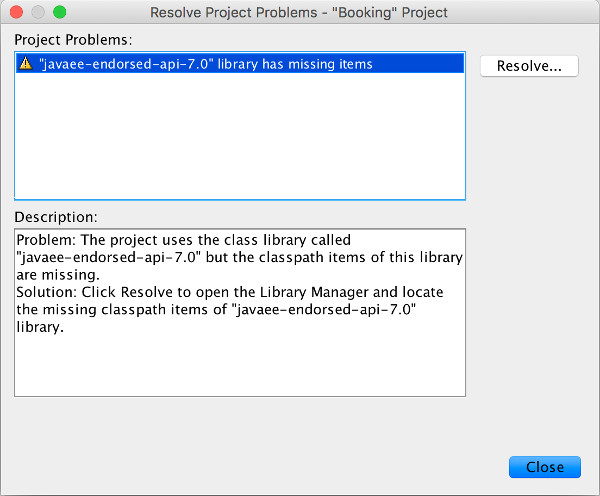
\includegraphics[scale=1]{img/instalacion/advertencia-javaee-endorsed-api.jpg}
  \caption{\textit{Advertencia de falta de librería javaee-endorsed-api-7.0}}
  \label{fig:advertencia-javaee-endorsed-api}
\end{figure}

\begin{figure}
\centering
  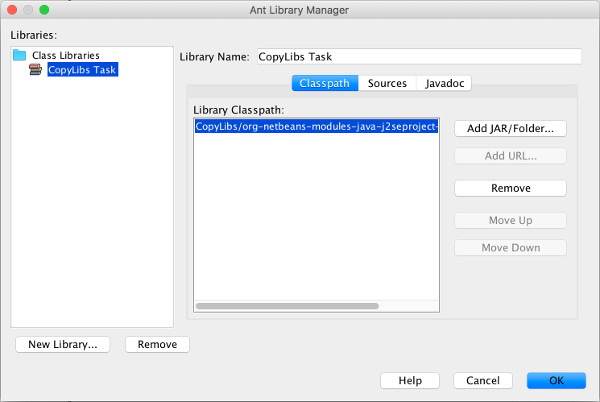
\includegraphics[scale=.85]{img/instalacion/resolver-javaee-endorsed-api.jpg}
  \caption{\textit{Resolver la dependencia de la librería javaee-endorsed-api-7.0}}
  \label{fig:resolver-javaee-endorsed-api}
\end{figure}

\item Prodeceremos ahora a la instalación de \textit{PostgreSQL} y \textit{pgAdmin} para su uso. Si no se crea un servidor por defecto, crearemos uno usando "\textit{localhost}" para el nombre y el \textit{host} y el resto de campos por defecto, como \textit{5432} para el puerto. 

\item Seguidamente crearemos un usuario dándole el nombre de "\textit{booking}".

\item Por último, crearemos nuestra base de datos "\textit{booking}", seleccionando al usuario con mismo nombre como propietario de la misma. 

\item A continuación realizaremos la carga de los datos de una base de datos básica. Para ello, haciendo clic secundario en la base de datos \textit{booking}, seleccionamos \textit{Restore...} y utilizamos la copia facilitada en el directorio \textit{db}. En el mismo, podemos consultar los datos de acceso para el sistema, así como un pequeño manual para crear nuevos administradores.

\item Antes de realizar la comprobación que todo está bien instalado y configurado, habrá que realizar la configuración del servidor de aplicaciones, en este caso \textit{GlassFish}.

\begin{enumerate}
\item Iniciaremos el servidor a través de \textit{NetBeans}. Para ello, navegaremos hasta la pestaña \textit{Services}, y expandiremos \textit{Servers}. Aquí, encontraremos nuestro servidor, haciendo clic derecho elegiremos la opción \textit{Start} para iniciarlo, como vemos en la figura \ref{fig:iniciar-glassfish}.

\begin{figure}[H]
\centering
  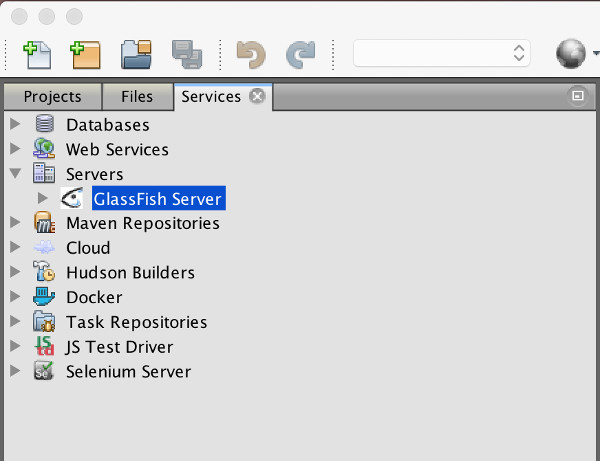
\includegraphics[scale=.95]{img/instalacion/iniciar-glassfish.jpg}
  \caption{\textit{Iniciando GlassFish}}
  \label{fig:iniciar-glassfish}
\end{figure}

\item Una vez finalizado de iniciar, podemos acceder a toda la configuración de \textit{GlassFish} -de acuerdo al archivo \textit{glassfish-resources.xml}, figura \ref{fig:glassfish-resources}- a través de nuestro navegador, haciendo uso del puerto 4848, accediendo mediante la URL: http://localhost:4848/ 
\item Configuraremos primero la conexión del servidor con la base de datos. Para ellos iremos a \textit{Resources > JDBC > JDBC Connection Pools}. Aquí añadiremos una nueva conexión a través del botón \textit{New...}. Aquí, le asignaremos un nombre y elegiremos el tipo de recurso y driver, como se muestra en la figura \ref{fig:new-connection-pool}. Además, se establecerán las propiedades de la base de datos como muestra la figura \ref{fig:connection-pool-properties}, de acuerdo a lo establecido en el archivo \textit{glassfish-resources.xml} que vemos en la imagen \ref{fig:glassfish-resources}.

\begin{figure}
\centering
  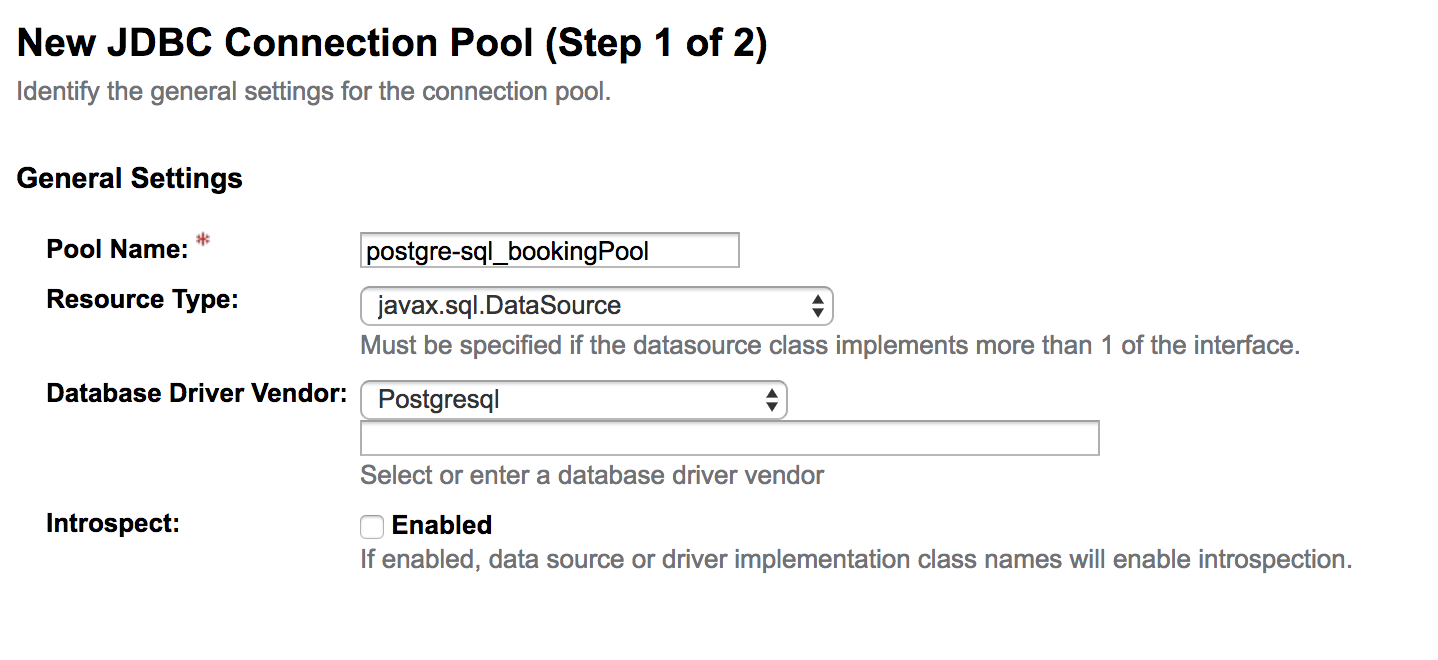
\includegraphics[scale=.45]{img/instalacion/new-connection-pool.png}
  \caption{\textit{Creando una nuevo conexión}}
  \label{fig:new-connection-pool}
\end{figure}

\begin{figure}
\centering
  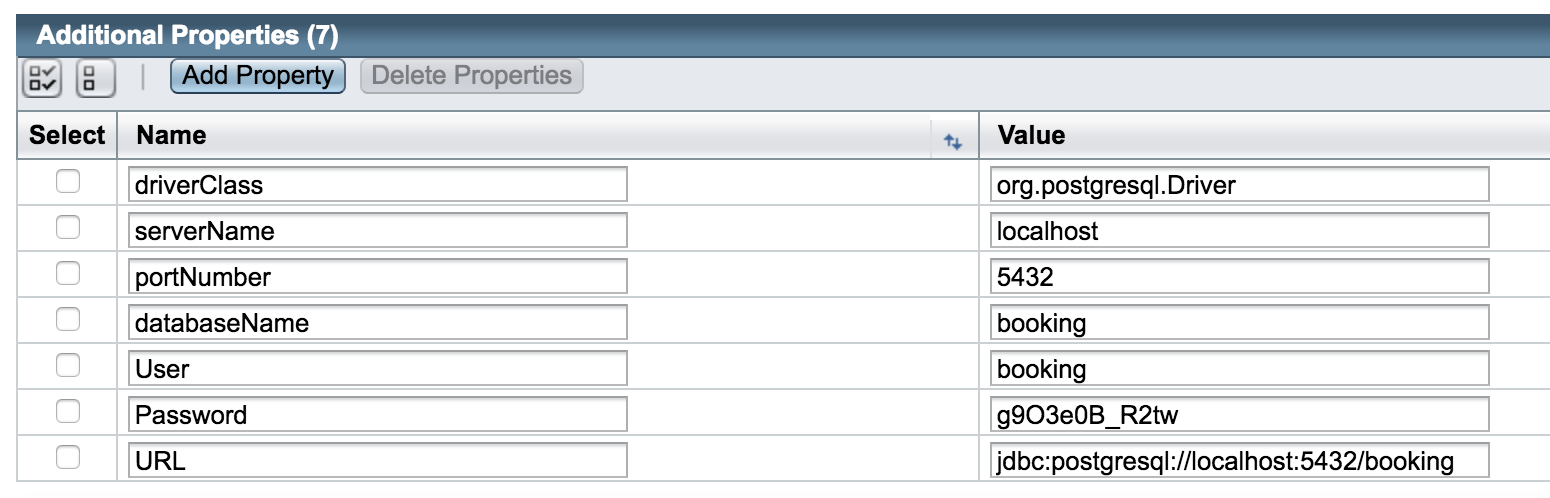
\includegraphics[scale=.45]{img/instalacion/connection-pool-properties.png}
  \caption{\textit{Añadiendo las propiedades de la conexión}}
  \label{fig:connection-pool-properties}
\end{figure}

\begin{figure}
\centering
  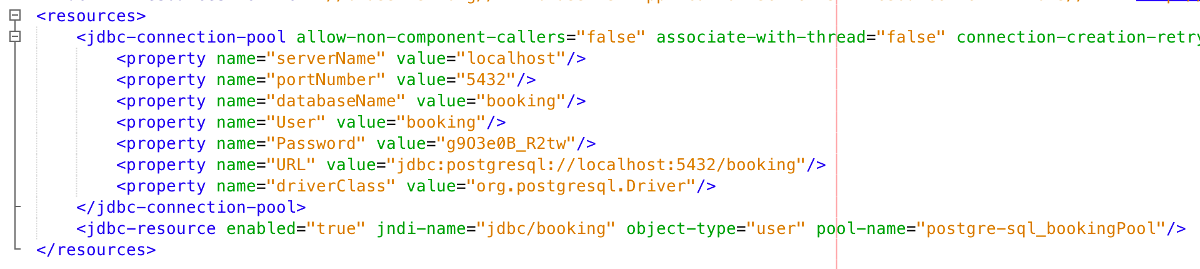
\includegraphics[scale=.70]{img/instalacion/glassfish-resources.png}
  \caption{\textit{Archivo glassfish-resources.xml}}
  \label{fig:glassfish-resources}
\end{figure}

\item A continuación, se crea el recurso \textit{JDBC (Java Database Connectivity)}. Para ello, navegaremos a \textit{JDBC Resources}, dentro del mismo nivel del menú, pulsamos el botón para crear uno nuevo, indicamos el nombre y elegimos la conexión creada previamente. 

\begin{figure}
\centering
  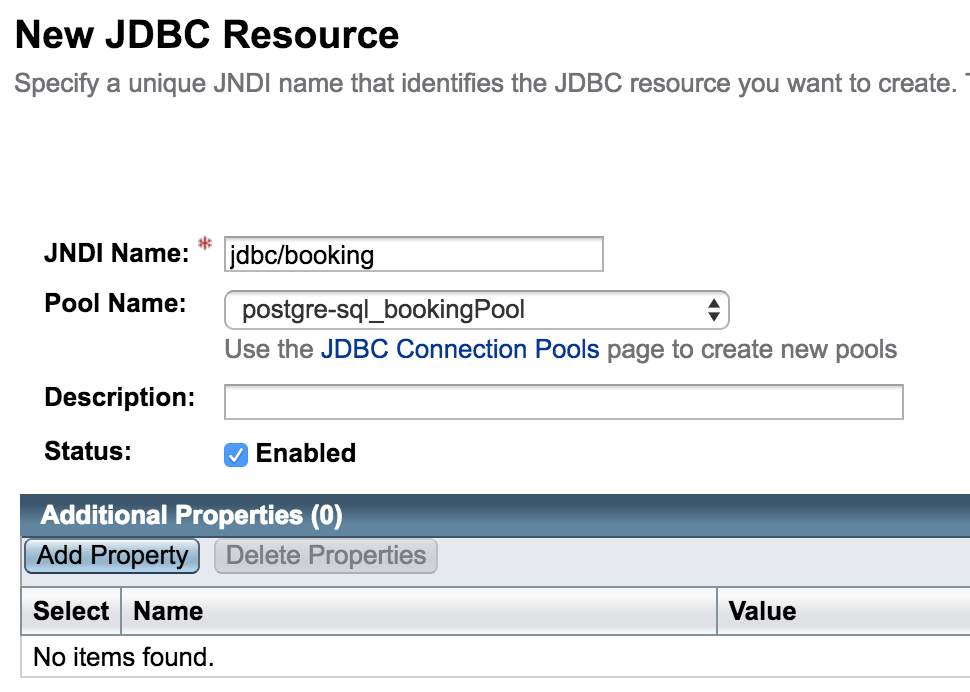
\includegraphics[scale=0.5]{img/instalacion/new-jdbc-resource.png}
  \caption{\textit{Creando un nuevo recurso JDBC}}
  \label{fig:new-jdbc-resource}
\end{figure}

\item Finalmente, para acabar la configuración, se especificará las tablas y columnas de la base de datos que se usarán para el control de sesiones de los usuarios en la aplicación. Para ello navegamos a \textit{Configurations > server-config > Security > Realms}. Añadiremos uno nuevo y especificaremos los datos necesarios para el uso del nombre de usuario y contraseña en las sesiones. La figura \ref{fig:new-realm} muestra los valores que usaremos para tal fin, qué tablas y columnas. Como vemos en la imagen, también añadiremos las propiedades necesarias, como hicimos anteriormente en la conexión con la BD.

\begin{figure}
\centering
  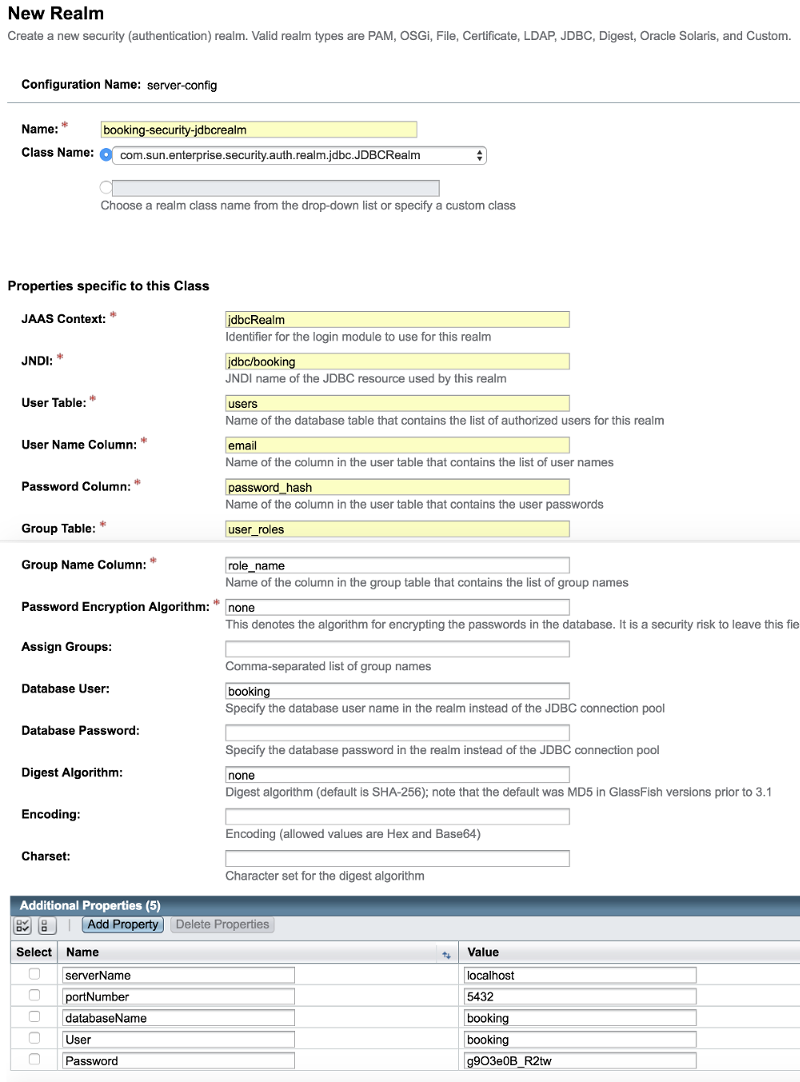
\includegraphics[scale=1]{img/instalacion/new-realm.png}
  \caption{\textit{Creando un nuevo ámbito para la seguridad de sesiones}}
  \label{fig:new-realm}
\end{figure}

\end{enumerate}

\item Por último, y antes de ejecutar el programa, añadiremos el archivo \textit{postgresql-9.3-1102.jdbc41.jar} al directorio \textit{glassfish > lib} dentro del directorio de \textit{GlassFish}.

\item Volviendo a \textit{NetBeans}, procedemos a comprobar que todo funciona correctamente compilando el proyecto (clic secundario al proyecto y seleccionamos \textit{Build}) y procediendo al \textit{deploy} (mismo procedimiento, clicando \textit{Deploy}). 

\item Una vez finalizado el proceso con éxito, abriremos el navegador web que usemos en nuestro equipo y accederemos a la aplicación mediante la URL \textit{localhost:8080}. 

\item Si todo ha ido bien, nos aparecerá la página de inicio de sesión. En caso que se produzca algún error podemos consultarlo en la ventana de \textit{GlassFish} del \textit{Output} de nuestro \textit{NetBeans}. Si se trata de un error que no se logre solucionar, puedes contactar con el autor, Jesús Soriano, a través de su web \cite{JesusSoriano}, del repositorio de \textit{GitHub} \cite{github-booking} o mediante correo electrónico: info@jesussoriano.com.
\end{enumerate}


\section{Pruebas de implantación}

Para comprobar que el sistema funciona correctamente, realizaremos pruebas básicas. 

\begin{itemize}
\item Para empezar, se procederá con el inicio de sesión de alguno de los usuarios que se facilitan.
\item A continuación, podemos realizar el registro de nuevos usuarios.
\item Una vez comprobado que esto se realiza correctamente, se puede hacer uso de las funcionalidades del sistema por parte tanto del superadministrador, como administrador y usuario. Como por ejemplo, creación de nuevos servicios o citas, subida de archivos, edición de perfiles, suspensión y activación de servicios y usuarios, reserva de plazas, comprobación de notificaciones, creación de noticias, etc. 
\item El proceso para realizar dichos ejemplos se puede consultar en el manual de usuario (capítulo \ref{sec:manual-usuario}).
\item Se recomienda la creación de usuarios reales para la utilización del sistema y no usar los que se facilitan como ejemplo. 
\item Si tenemos problemas con los datos de la BD, podemos comprobar si la conexión con la misma se hace correctamente a través de la pestaña \textit{Services}, desplegando \textit{Databases} y probando si nuestra base de datos (que debería estar listada al desplegar) conecta adecuadamente haciendo clic secundario y eligiendo la primera opción para conectar.
\end{itemize}


\section{Procedimientos de operación y nivel de servicio}

Si se realizan modificaciones o ampliaciones de requisitos del sistema, se recomienda que se trabaje siempre guardando una copia de seguridad tras la finalización de un nuevo componente o modificación de uno existente. En este PFC se ha trabajado usando \textit{GitHub} como repositorio \textit{Git}. También es recomendable guardar un backup de la base de datos cada cierto tiempo, o cuando los datos son sólidos, por si hubiese algún problema con la misma o se requiera una nueva instalación del sistema. \\

En caso de usarse el sistema en producción, los backups de base de datos serían casi de carácter obligatorio para evitar la pérdida de datos de usuarios reales. 

